% !TEX encoding = UTF-8
% !TEX TS-program = pdflatex
% !TEX root = ../tesi.tex

%**************************************************************
\chapter{Il contesto aziendale}

\section{L'azienda}

Siav è una delle più importanti realtà italiane di sviluppo software e di servizi informatici
specializzata nella dematerializzazione e nella gestione documentale e nei processi
digitali. Presenta diverse filiali nel suolo italiano che cooperano tra loro per un fine comune. Siav inoltre punta molto sulla collaborazione tra aziende, in campo nazionale sia a livello pubblico che privato, ma anche a livello internazionale. Una fra tutti Microsoft.
I loro servizi puntano ad una miglior gestione, controllo ed automazione di tutti i principali processi aziendali.
\begin{figure}[!h] 
	\centering 
	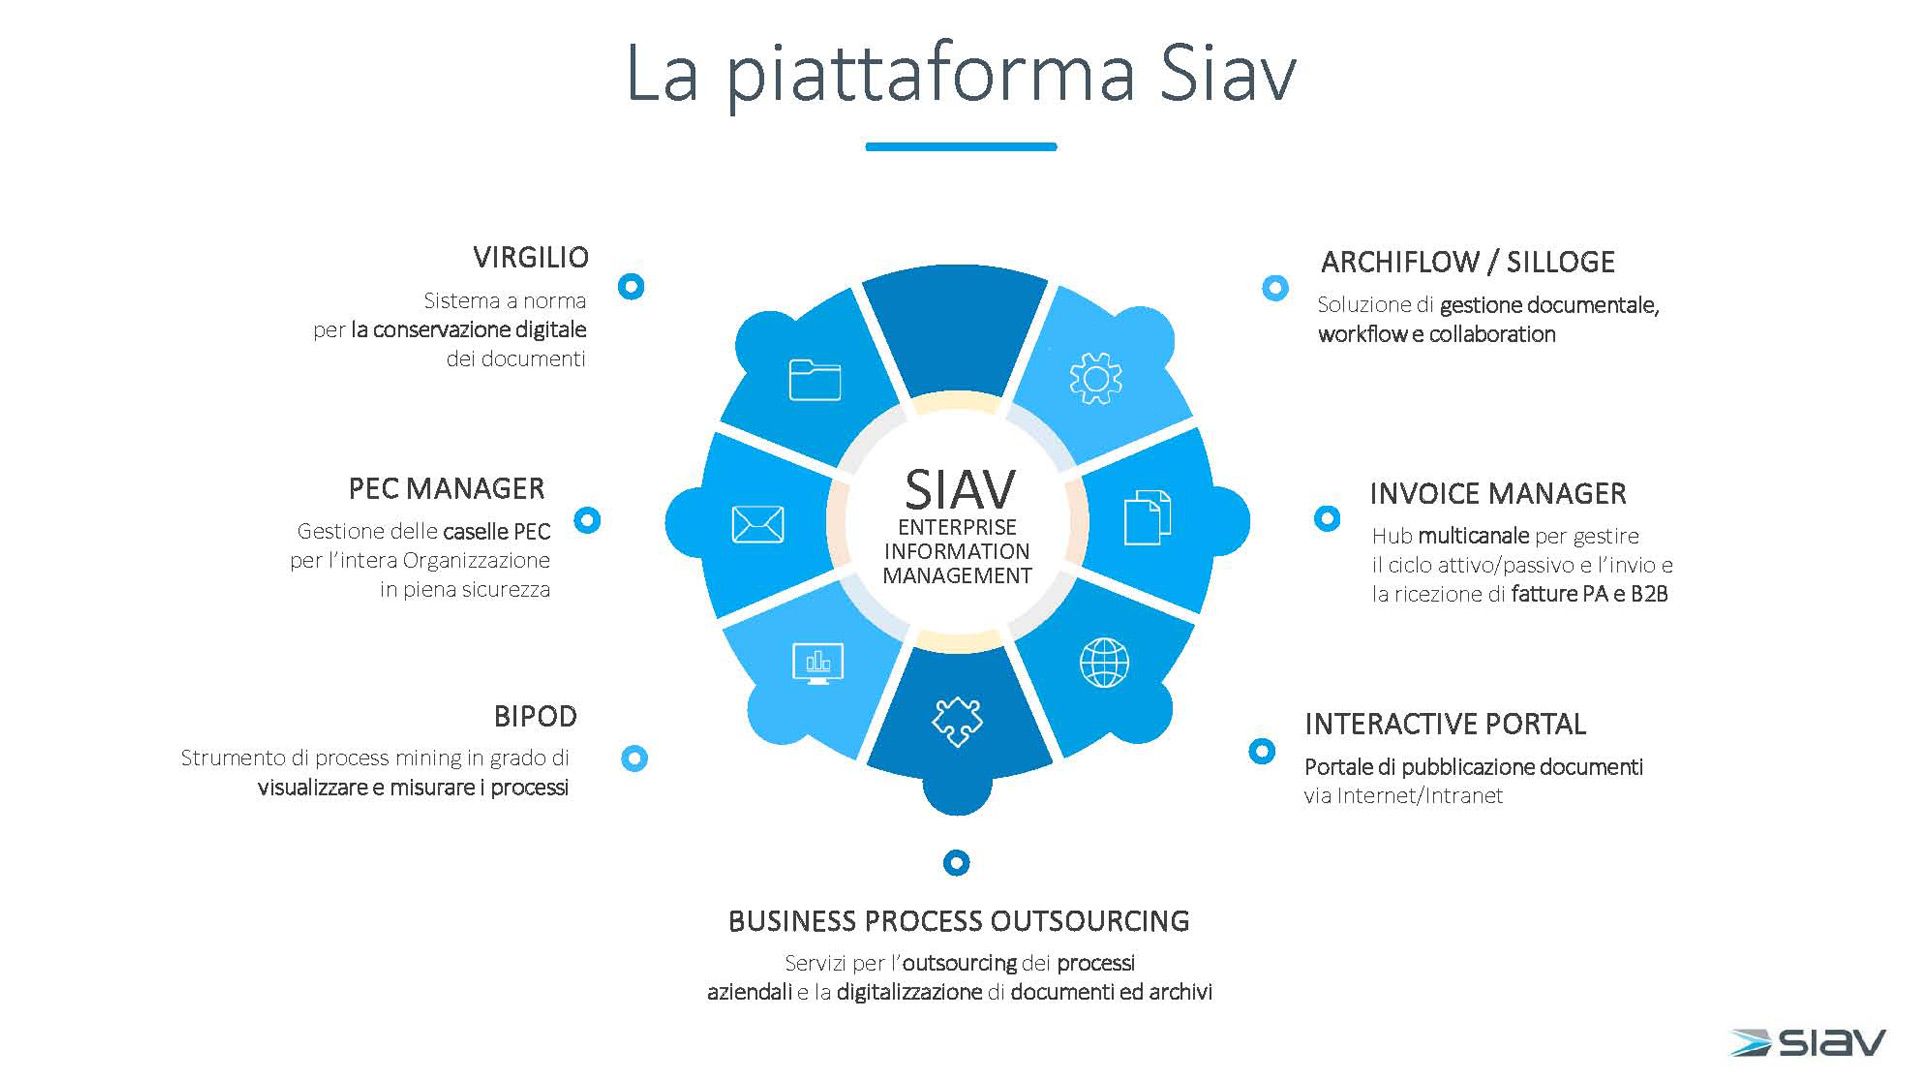
\includegraphics[width=1.1\columnwidth]{siav} 
	\caption{I prodotti offerti da Siav}
\end{figure}

\section {Dominio Applicativo}
Siav si colloca all'interno del mercato come una tra la più importanti realtà italiane a livello di \textit{Enterprise Content Management} offrendo servizi per poter migliorare processi e gestioni aziendali spaziando da un gestore di caselle PEC, ad un applicativo di process mining denominato Bipod, fino ad arrivare al loro prodotto di punta: Archiflow/Silloge: un software in continuo sviluppo, mantenuto e aggiornato da piccoli team che lavorano in sinergia per raggiungere un obiettivo comune. Archiflow/Silloge offre una soluzione alla gestione di una cospicua mole di documenti, categorizzandoli in varie sezioni permettendone un facile reperimento.

\section {Tecnologie utilizzate}
Le tecnologie utilizzate dell'azienda per la realizzazione dei propri prodotti sono fondate principalmente sulla possibilità di un utilizzo tramite cloud. Si sono dedicati principalmente sullo sviluppo di \textit{Webapp}. Tali tecnologie possono essere raggruppate in due macrocategorie: \textit{Frontend} e \textit{Backend}.
\subsection{\textit{Frontend}}
Da quel che ho potuto constatare durante l'attività di stage, per quanto riguarda lo sviluppo web lato \textit{client} viene utilizzato prevalentamente Angular. Tramite il consistente numero di componenti prefabbricati presenti in rete e una vasta gamma di funzionalità e servizi disponibili, è possibile sviluppare un'interfaccia frontend di qualità a proprio piacimento, soddisfando nel miglior modo possibile le aspettative del cliente.
\begin{figure}[!h] 
	\centering 
	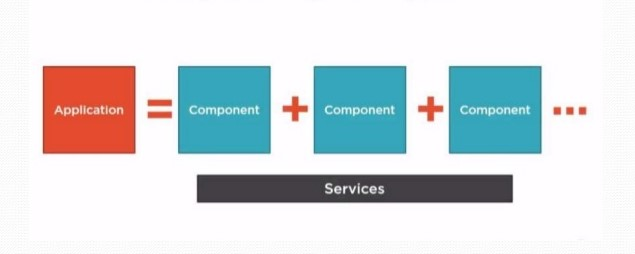
\includegraphics[width=0.8\columnwidth]{angular} 
	\caption{Esempio di struttura di un applicativo Angular}
\end{figure}
\subsection{\textit{Backend}}
Per quanto riguarda lato backend vengono utilizzate molteplici tecnologie in base al software di sviluppo in esame: 
All'interno del loro software di punta Archiflow/Silloge viene utilizzato \textit{Kafka}. Tale sistema consente la gestione di un elevato numero di operazioni in tempo reale per un numero elevato di \textit{client}. Quest'ultimo gestore offre la possibilità di monitorare le attività web memorizzando ed inviando flussi di dati in tempo reale. La tematica dei flussi è molto delicata per il software Archiflow, dovendo gestire una grande mole di documenti ed essendo utilizzato da un cospicuo numero di utenti.
\begin{figure}[!h] 
	\centering 
	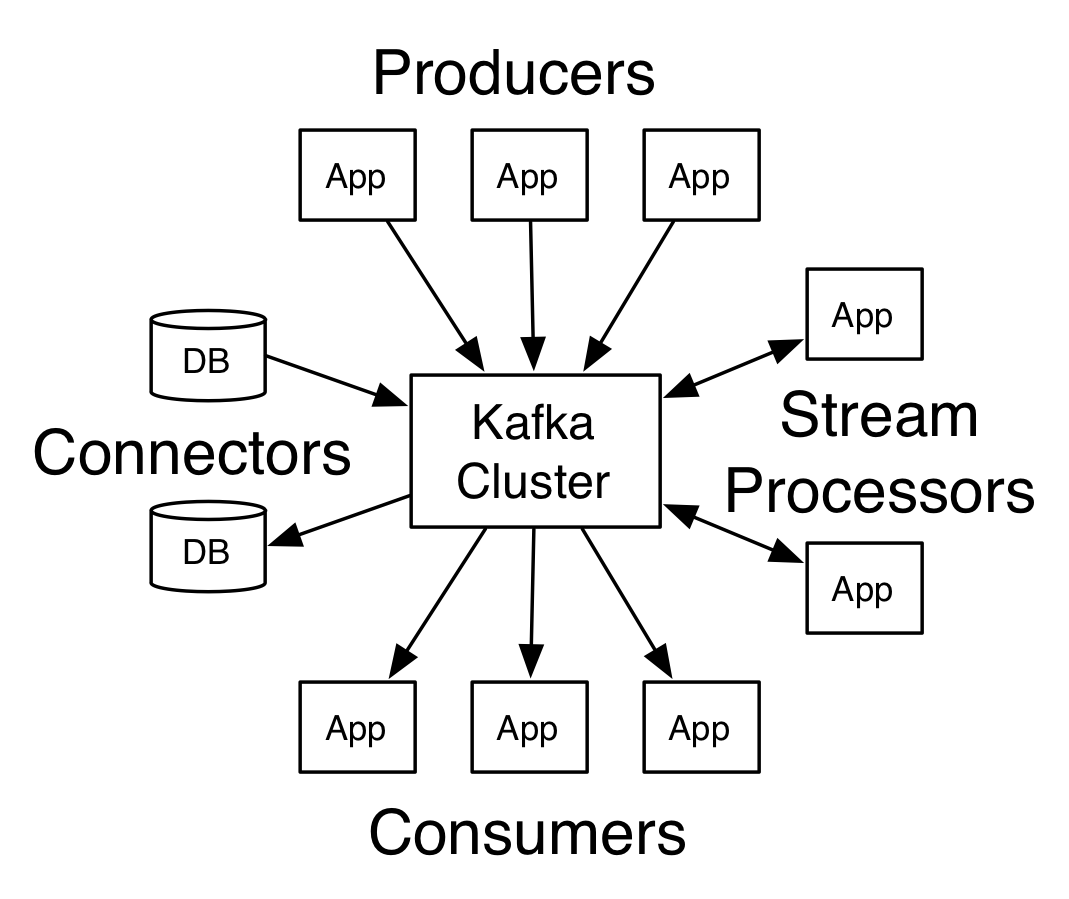
\includegraphics[width=0.8\columnwidth]{kafka} 
	\caption{Diagramm illustrativo sul funzionamento di Apache Kafka}
\end{figure}
\section {Processi aziendali}
\subsection{Metodologie si sviluppo}
L'azienda normalmente si ritrova a dover far fronte ad alcune problematiche derivate da bug, criticità o variazioni importanti di requisiti che possono essere riscontrate durante i vari processi aziendali ed incidere in modo significativo sull'andamento dello sviluppo.
Per cercare di venire incontro a ciò l'azienda ha adottato una metodologia di tipo \textit{Agile}, cercando di mantenere un atteggiamento flessibile rispetto ai processi e gli obiettivi. Risulta quindi fondamentale l'organizzazione di incontri durante vari momenti della giornata o settimana in modo da confrontarsi sull'andamento dei processi e lo stato di avanzamento del prodotto. È consuetudine dei team di lavoro un confronto giornaliero tramite \textit{daily meeting}, per discutere su quanto fatto durante la giornata precedente indicando le eventuali criticità riscontrate, pianificando cosi gli obiettivi per la giornata odierna. Ad inizio settimana invece viene organizzato \textit{weekly meeting} per constatare gli stati di avanzamento rispetto alla settimana precedente, per poi fissare gli obiettivi per la settimana successiva.
Qui di seguito sono riportati i principi cardine del Manifesto Agile:
\begin{itemize}
	\item La nostra massima priorità è soddisfare il cliente
	rilasciando software di valore, fin da subito
	e in maniera continua. 
	\item Accogliamo i cambiamenti nei requisiti,
	anche a stadi avanzati dello sviluppo.
	I processi \textit{Agile} sfruttano il cambiamento
	a favore del vantaggio competitivo del cliente. 
	\item Consegniamo frequentemente software funzionante,
	con cadenza variabile da un paio di settimane a un paio di mesi,
	preferendo i periodi brevi. 
	\item Committenti e sviluppatori devono lavorare insieme
	quotidianamente per tutta la durata del progetto. 
	\item Fondiamo i progetti su individui motivati.
	Diamo loro l'ambiente e il supporto di cui hanno bisogno
	e confidiamo nella loro capacità di portare il lavoro a termine. 
	\item Una conversazione faccia a faccia
	è il modo più efficiente e più efficace per comunicare
	con il team ed all'interno del team. 
	\item Il software funzionante è il principale metro di misura di progresso. 
	\item I processi agili promuovono uno sviluppo sostenibile.
	Gli sponsor, gli sviluppatori e gli utenti dovrebbero essere in grado
	di mantenere indefinitamente un ritmo costante. 
	\item La continua attenzione all'eccellenza tecnica
	e alla buona progettazione esaltano l'agilità. 
	\item La semplicità - l'arte di massimizzare la quantità
	di lavoro non svolto - è essenziale. 
	\item Le architetture, i requisiti e la progettazione
	migliori emergono da team che si auto-organizzano. 
	\item A intervalli regolari il team riflette su come
	diventare più efficace, dopodiché regola e adatta
	il proprio comportamento di conseguenza. 
\end{itemize}
\begin{figure}[!h] 
	\centering 
	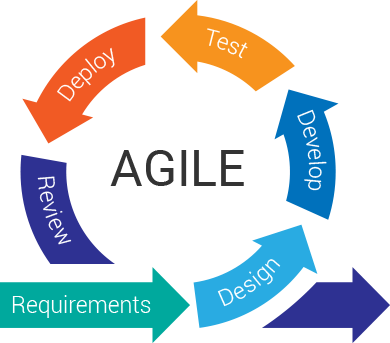
\includegraphics[width=0.4\columnwidth]{agile} 
	\caption{Ciclo di vita della metodologia Agile}
\end{figure}
\subsection{Strumenti di supporto}
\paragraph{Gestione di progetto:}
Per tenere traccia del lavoro svolto e delle modifiche apportate viene utilizzato \textit{Evernote}: un software che permette la scrittura e la condivisione di note ad un gruppo cospicuo di utenti. Cosi facendo ogni membro del team di sviluppo ha sotto controllo ogni attività svolta dagli altri membri.
Un ulteriore strumento utilizzato per il tracciamento dello attività è \textit{Google Docs}, ma al contrario di \textit{Evernote}, è possbilie assegnare task agli utenti che hanno i permessi di accesso al documento. Solitamente i task assegnati presentano una struttura tanto semplice quanto incisiva: è presente innanzitutto la data di creazione, la possibilità o meno di menzionare direttamente l'interessato a cui risulta assegnato il task ed un casella di risposta per poter descrivere la sua effettiva terminazione, oppure un messaggio di testo di altro genere, che solitamente indica le problematiche per cui il task non è stato possibile risolverlo. 
\paragraph{Ambienti di sviluppo}
Gli ambienti di sviluppo adottati in Siav sono vari. Non è presente una direttiva specifica che indica gli \textit{editor} e i compilatori da utilizzare. Solitamente, per lo sviluppo di interfacce web viene utilizzato \textit{Visual Studio Code}: permette la creazione di più terminali all'interno della stessa sessione in modo da poter effettuare diverse operazioni in modo simulataneo. Oltre a questo permette una visualizzazione semplficiata delle modifiche apportate al repository, offrendo la possibilità di effettuare tutte le principale operazioni di \textit{Git}.
Per quanto riguarda lo sviluppo di applicativi in \textit{Python} viene spesso utilizzato \textit{PyCharm}, mentre per lo sviluppo in ambiente \textit{Java} viene utilizzato \textit{IntelliJ IDEA} oppure \textit{Eclipse}, ma anche \textit{Subilme text} è risultata una valida alternativa.  
\paragraph{Controllo versionamento:}
Come strumento di versionamento l'azienda utilizza Git. In particolare viene utilizzata una versione \textit{Enterprise} di \textit{gitLab} con un dominio interno all'azienda. Non risulta quindi possibile l'esportazione di un repository al di fuori di questa. Ciò garantisce una sicurezza in più rispetto ai repository utilizzati per scopo accademico.
I principali aspetti che hanno portato l'azienda all'utilizzo sono:
\begin{itemize}
	\item \textit{branch/merge:} Permette con facilità la creazione di \textit{branch}, in modo che ogni sviluppatore possa lavorare nel proprio ramo senza intaccare quello principale (stabile) del rapository, evitando quindi la generazioni di conflitti o errori. Nel momento in cui il software sviluppato all'interno branch viene definito stabile è possibile riallinearlo con il ramo principale tramite un'operazione di \textit{merge}.
	\item Reperibilità: Anche in assenza di connessione è possibile effettuare commit in locale, in modo da non perdere i progressi fatti finora e salvare il lavoro fatto.
	\item Ridondanza: Ogni Sviluppatore contiene una copia del repository: Il rischio di perdita dei dati è dunque diviso tra i \textit{contributors} che possiedono l'ultima versione del software in locale.
\end{itemize} 
\section{Clientela rivolta a Siav}
La maggior parte dei clienti che si affidano a Siav sono aziende che presentano il bisogno di automatizzarsi o migliorare i propri processi interni andando cosi ad incrementare la propria efficenza sotto l'aspetto lavoartivo. Tali aziende sono di vario genere, dal semplice ristorante ad una nota catena di supermercati fino ad aziende metalmeccaniche. Per ogni settore, Siav offre diverse opportunità di gestione e miglioramento aziendale.
Siav è catalogata come \textit{Software house} e presenta un ampio catalogo di prodotti atti a soddisfare le principali necessità organizzative di un'azienda, sta al potenziale cliente poi, valutarne l'acquisto in base alle proprie necessità. 
\section{Propensione all'innovazione}
Siav è in costante crescita ed è in continua ricerca di nuove tecnologie da implementare all'interno dei propri prodotti. Presentano un ottimo reparto di Ricerca e Sviluppo nel quale sono costantemente impegnati in nuove tematiche da affrontare facedo sempre riferimento ai bisogni dei clienti. Essendo, quello dell'informatica, un settore in continua crescita è necessario che il team di Ricerca e Sviluppo operi costantemente al fine di trovare nuove risorse e tecnologie da affrontare e sperimentare. Una cospicua fetta di questi studi e approfondimenti vengono concretizzati tramite progetti sperimentali e attività di stage, in modo da poter osservare nel concreto se tali ricerche possano produrre risultati che giovino all'azienda. 